\chapter{Testy i porównanie algorytmów}
\section{Analiza działania poszczególnych algorytmów}
\subsection{Algorytm Roju Cząsteczek}
\subsection{Algorytm Adaptacyjny Tabu}
Przedstawienie działania algorytmu dla wybranych testów.
\par \textbf{Test 1}
\begin{figure}[H]
  \caption{Wykres zależności funkcji oceny od czasu}
  \centering
    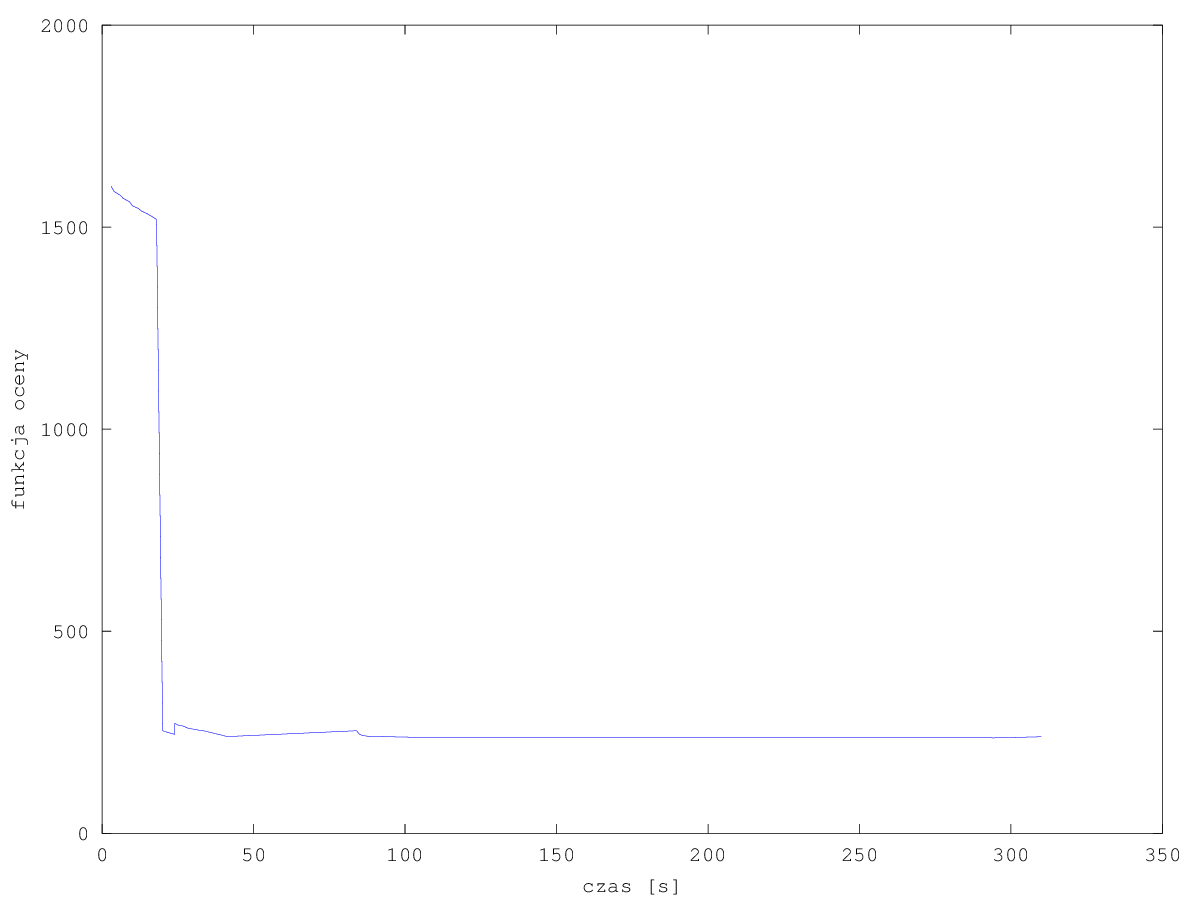
\includegraphics[width=0.8\textwidth]{ogolny.png}
\end{figure}
\begin{figure}[H]
  \caption{Wykres zależności funkcji oceny od czasu, bez uwzględnienia fazy inicjalizacji}
  \centering
    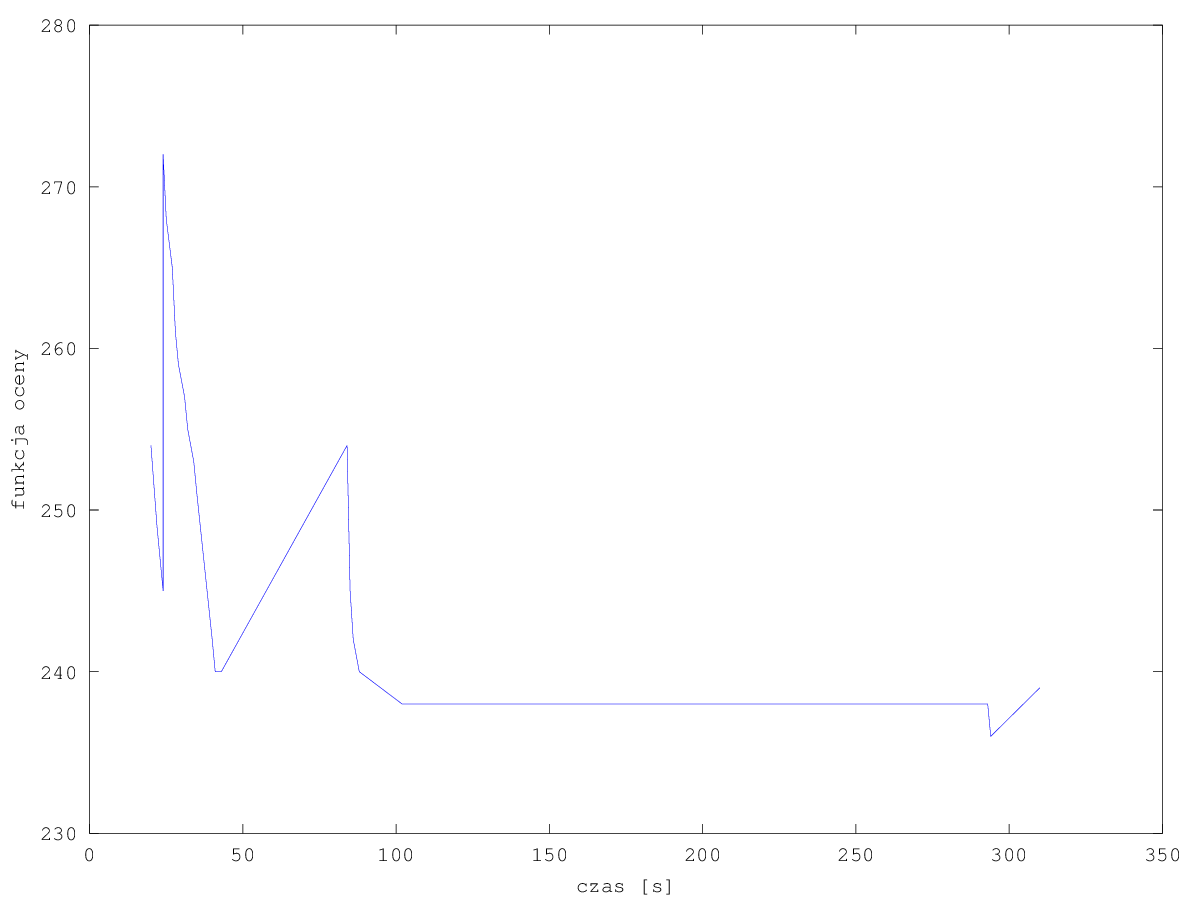
\includegraphics[width=0.8\textwidth]{szczeg.png}
\end{figure}
\par \textbf{Test 2}
\begin{figure}[H]
  \caption{Wykres zależności funkcji oceny od czasu}
  \centering
    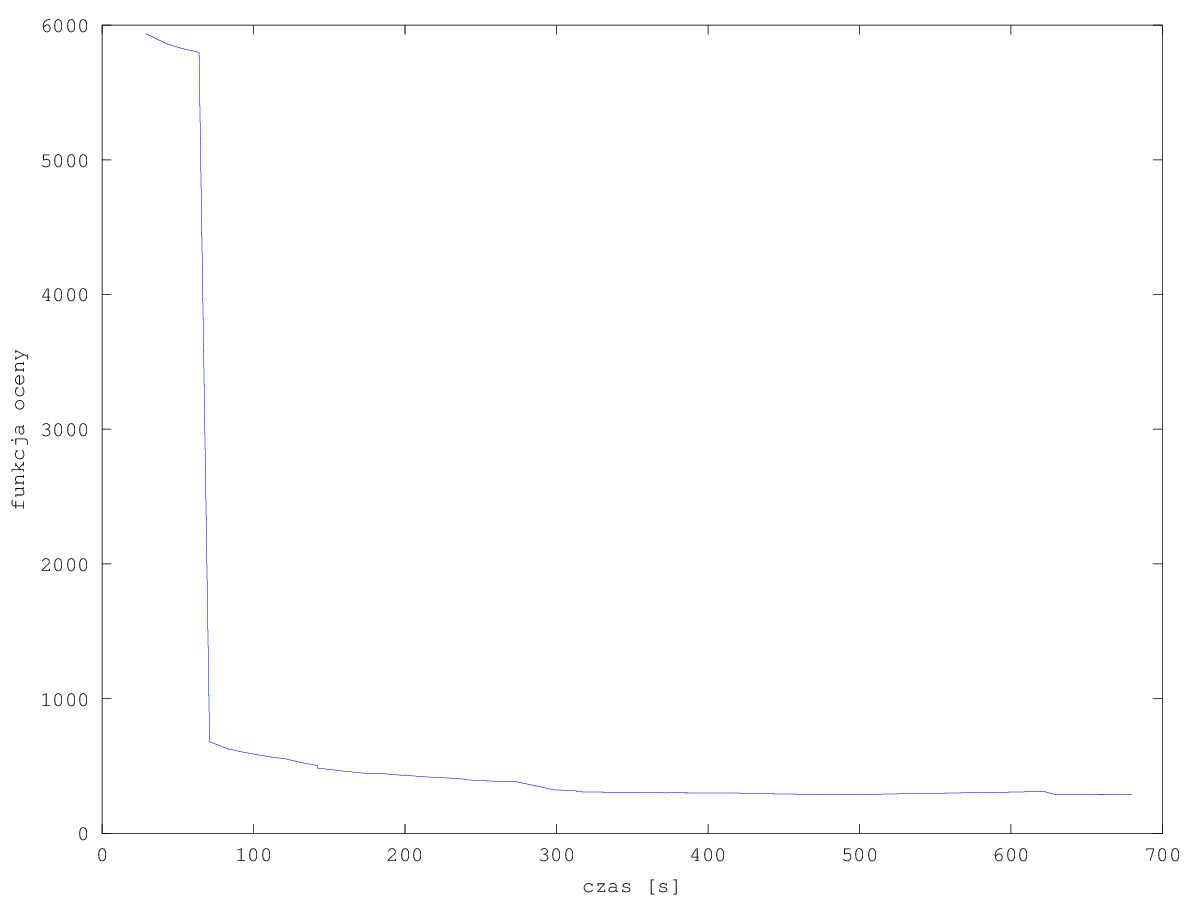
\includegraphics[width=0.8\textwidth]{ogolny2_instancja.png}
\end{figure}
\begin{figure}[H]
  \caption{Wykres zależności funkcji oceny od czasu, bez uwzględnienia fazy inicjalizacji}
  \centering
    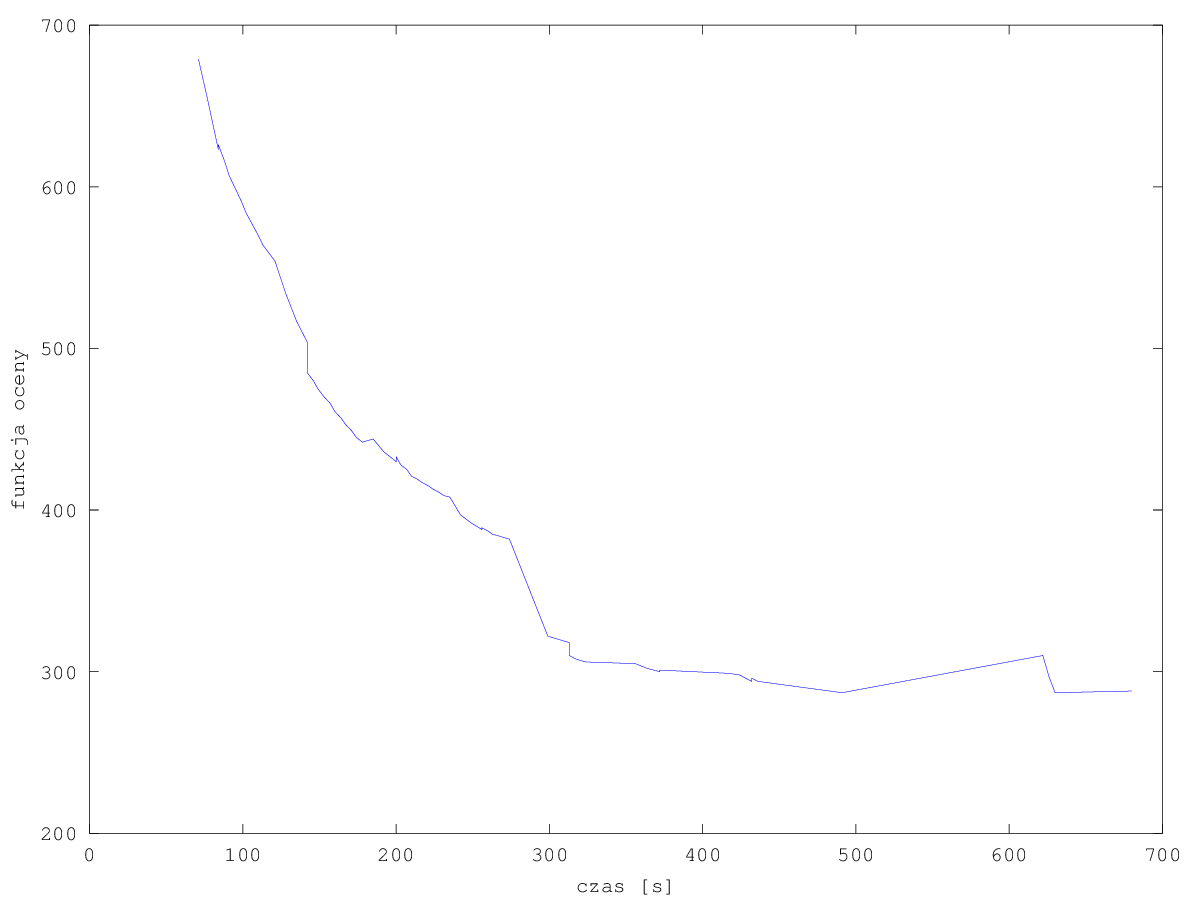
\includegraphics[width=0.8\textwidth]{szczegolowy2_instancja.png}
\end{figure}
\subsection{Algorytm Genetyczny}
\section{Specyfikacja testów}
Dane testowe pobrane zostały z konkursu ,,International Timetabling Competition 2007''. Do oceny rozwiązań używany jest oryginalny walidator rozwiązań, zapewniony przez organizatorów konkursu.
\subsection{Test 1}
\begin{table}[H]
\begin{center}
 
\begin{tabular}{ |l|l| }
\hline
$Liczba\ kursów$ & $30$\\
\hline
$Liczba\ programów\ nauczania$ & $14$\\
\hline
$Liczba\ dni$ & $5$ \\
\hline
$Licza\ przedziałów\ czasowych$ & $6$ \\
\hline
$Liczba\ ograniczeń$ & $53$ \\
\hline
$Liczba\ sal$ & $6$ \\
\hline
\end{tabular}
\end{center}
\end{table}
\par Wyniki działania algorytmów- ocena wygenerowanych planów zajęć: \\
Parametry dla algorytmów:
\begin{enumerate}
\item GA - liczba osobników: 100, liczba iteracji: 500, szacowany czas działania algorytmu: 150 s
\item PSO - liczba cząsteczek: 20, liczba iteracji 10000, szacowany czas działania algorytmu: 40 min
\item ATS - czas działania: 120 s
\end{enumerate}
\begin{table}[H]
\begin{center}

\begin{tabular}{ |l|l|l|l| }
\hline
 & $GA$ & $PSO$ & $ATS$\\
\hline
${H}_{1}\ Wykłady$ & $0$ & $0$ & $0$\\
\hline
$H_{2}\ Zajętość\ sali$ & $0$ & $0$ & $0$\\
\hline
$H_{3}\ Konflikty\ pomiędzy\ kursami$ & $0$ & $0$ & $0$ \\
\hline
$H_{4}\ Dostępność\ wykładowcy$ & $0$ & $0$ & $0$ \\
\hline
$S_{1}\ Wielkość\ sali$ & $4$ & $5$ & $205$ \\
\hline
$S_{2}\ Stabilność\ pomieszczenia$ & $14$ & $24$ & $32$ \\
\hline
$S_{3}\ Minimalna\ liczba\ dni$ & $0$ & $0$ & $0$ \\
\hline
$S_{4}\ Zwartość\ zajęć$ & $56$ & $8$ & $6$ \\
\hline
$Funkcja\ oceny$ & $74$ & $37$ & $243$ \\
\hline
\end{tabular}
\end{center}
\caption {Wyniki uzyskane przez poszczególne algorytm}
\end{table}
\subsubsection{Test 1 - wizualizacja}
\begin{figure}[H]
  \caption{Graf przedstawiający wszystkie zależności pomiędzy kursami (uwzględniając tych samych prowadzących nauczycieli oraz należenie kursu do tego samego programu nauczania) }
  \centering
    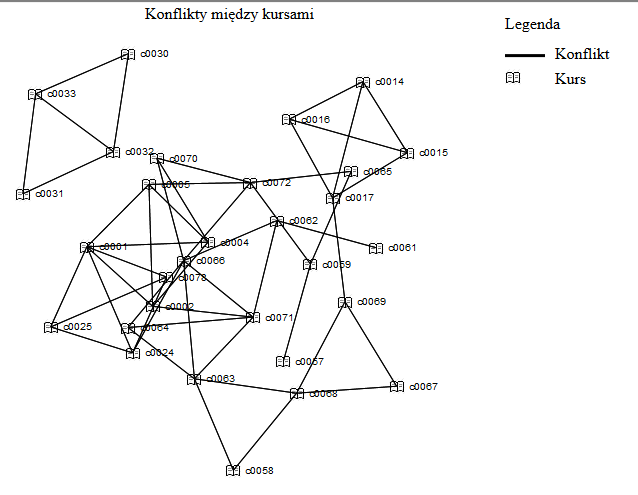
\includegraphics[width=0.8\textwidth]{test1.PNG}
\end{figure}


\begin{figure}[H]
  \caption{Graf uwzględniający zależności pomiędzy kursami uwzględniając prowadzących dane kursy}
  \centering
    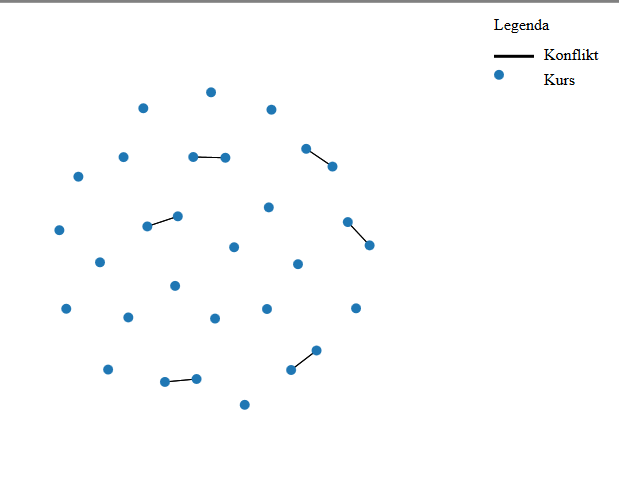
\includegraphics[width=0.8\textwidth]{test1_teach.PNG}
\end{figure}
\begin{figure}[H]
  \caption{Graf uwględniający grupy zależnych od siebie kursów wchodzących w skład tego samego programu nauczania}
  \centering
    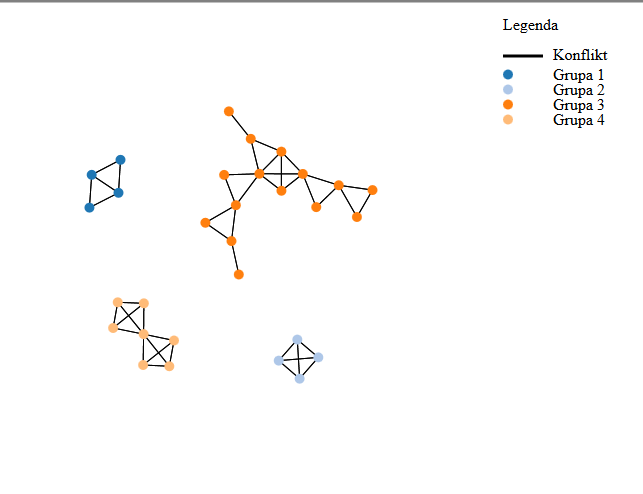
\includegraphics[width=0.8\textwidth]{test1_con.PNG}
\end{figure}
\subsection{Test 2}
\begin{table}[H]
\begin{center}

\begin{tabular}{ |c|c|c|c| }
\multicolumn{1}{r}{}
 &  \multicolumn{1}{c}{$$}
 & \multicolumn{1}{c}{$$} 
 \\
\cline{1-2}
$Liczba\ kursów$ & $82$\\
\cline{1-2}
$Liczba\ programów\ nauczania$ & $70$\\
\cline{1-2}
$Liczba\ dni$ & $5$ \\
\cline{1-2}
$Licza\ przedziałów\ czasowych$ & $5$ \\
\cline{1-2}
$Liczba\ ograniczeń$ & $513$ \\
\cline{1-2}
$Liczba\ sal$ & $16$ \\
\cline{1-2}
\end{tabular}
\end{center}
\caption {Specyfikacja danych - Test 2}
\end{table}
\par Wyniki działania algorytmów- ocena wygenerowanych planów zajęć: \\
Parametry dla algorytmów:
\begin{enumerate}
\item GA - liczba osobników: 200, liczba iteracji: 1000, szacowany czas działania algorytmu: 33 min
\item PSO - liczba cząsteczek: 20, liczba iteracji 10000, szacowany czas działania algorytmu: 180 min
\item ATS - czas działania: 480 s
\end{enumerate}
\begin{table}[H]
\begin{center}

\begin{tabular}{ |l|l|l|l| }
\hline
 & $GA$ & $PSO$ & $ATS$\\
\hline
${H}_{1}\ Wykłady$ & $0$ & $1$ & $0$\\
\hline
$H_{2}\ Zajętość\ sali$ & $0$ & $0$ & $0$\\
\hline
$H_{3}\ Konflikty\ pomiędzy\ kursami$ & $0$ & $0$ & $0$ \\
\hline
$H_{4}\ Dostępność\ wykładowcy$ & $0$ & $2$ & $0$ \\
\hline
$S_{1}\ Wielkość\ sali$ & $119$ & $54$ & $0$ \\
\hline
$S_{2}\ Stabilność\ pomieszczenia$ & $63$ & $51$ & $143$ \\
\hline
$S_{3}\ Minimalna\ liczba\ dni$ & $70$ & $74$ & $40$ \\
\hline
$S_{4}\ Zwartość\ zajęć$ & $424$ & $150$ & $104$ \\
\hline
$Funkcja\ oceny$ & $676$ & $330$ & $287$ \\
\hline
\end{tabular}
\end{center}
\caption {Wyniki uzyskane przez poszczególne algorytmy}
\end{table}
\subsection{Test 3}
\begin{table}[H]
\begin{center}

\begin{tabular}{ |c|c|c|c| }
\multicolumn{1}{r}{}
 &  \multicolumn{1}{c}{$$}
 & \multicolumn{1}{c}{$$} 
 \\
\cline{1-2}
$Liczba\ kursów$ & $72$\\
\cline{1-2}
$Liczba\ programów\ nauczania$ & $68$\\
\cline{1-2}
$Liczba\ dni$ & $5$ \\
\cline{1-2}
$Licza\ przedziałów\ czasowych$ & $5$ \\
\cline{1-2}
$Liczba\ ograniczeń$ & $382$ \\
\cline{1-2}
$Liczba\ sal$ & $16$ \\
\cline{1-2}
\end{tabular}
\end{center}
\caption {Specyfikacja danych - Test 3}
\end{table}
\par Wyniki działania algorytmów- ocena wygenerowanych planów zajęć: \\
Parametry dla algorytmów:
\begin{enumerate}
\item GA - liczba osobników: 200, liczba iteracji: 1000, szacowany czas działania algorytmu: 33 min
\item PSO - liczba cząsteczek: 20, liczba iteracji 5000, szacowany czas działania algorytmu: 90 min
\item ATS - czas działania: 16min
\end{enumerate}
\begin{table}[H]
\begin{center}

\begin{tabular}{ |l|l|l|l| }
\hline
 & $GA$ & $PSO$ & $ATS$\\
\hline
${H}_{1}\ Wykłady$ & $0$ & $0$ & $0$\\
\hline
$H_{2}\ Zajętość\ sali$ & $0$ & $0$ & $0$\\
\hline
$H_{3}\ Konflikty\ pomiędzy\ kursami$ & $0$ & $0$ & $0$ \\
\hline
$H_{4}\ Dostępność\ wykładowcy$ & $0$ & $1$ & $0$ \\
\hline
$S_{1}\ Wielkość\ sali$ & $82$ & $109$ & $12$ \\
\hline
$S_{2}\ Stabilność\ pomieszczenia$ & $50$ & $57$ & $125$ \\
\hline
$S_{3}\ Minimalna\ liczba\ dni$ & $20$ & $70$ & $40$ \\
\hline
$S_{4}\ Zwartość\ zajęć$ & $412$ & $202$ & $102$ \\
\hline
$Funkcja\ oceny$ & $564$ & $438$ & $279$ \\
\hline
\end{tabular}
\end{center}
\caption {Wyniki uzyskane przez poszczególne algorytmy}
\end{table}
\par PSO nie usuwan hardów (wybrana metoda nie odporna na lokane minima), . Ostateczne rozw jest najprostsze - to slabo dziala
\par badawczo 
GA - niepewne rozw element losow (roznie generuje poczatkowe rozwiazania), duza liczba osobnikow, upodobniaja zwiekszenie wspolczynnika mutacji do wyjscia z lokalnego minimum
\par system prosty do wykorzystania alg, otwarty na rozbudowe: rezcna edycja planu, wprowadzenie przez nuczycieli 






